\let\negmedspace\undefined
\let\negthickspace\undefined
\documentclass[journal]{IEEEtran}
\usepackage[a5paper, margin=10mm, onecolumn]{geometry}
%\usepackage{lmodern} % Ensure lmodern is loaded for pdflatex
\usepackage{tfrupee} % Include tfrupee package

\setlength{\headheight}{1cm} % Set the height of the header box
\setlength{\headsep}{0mm}     % Set the distance between the header box and the top of the text

\usepackage{gvv-book}
\usepackage{gvv}
\usepackage{cite}
\usepackage{amsmath,amssymb,amsfonts,amsthm}
\usepackage{algorithmic}
\usepackage{graphicx}
\usepackage{textcomp}
\usepackage{xcolor}
\usepackage{txfonts}
\usepackage{listings}
\usepackage{enumitem}
\usepackage{mathtools}
\usepackage{gensymb}
\usepackage{comment}
\usepackage[breaklinks=true]{hyperref}
\usepackage{tkz-euclide}
\usepackage{listings}                                     
\def\inputGnumericTable{}                                 
\usepackage[utf8]{inputenc}                                
\usepackage{color}                                            
\usepackage{array}                                            
\usepackage{longtable}                                       
\usepackage{calc}                                             
\usepackage{multirow}                                         
\usepackage{hhline}                                           
\usepackage{ifthen}                                           
\usepackage{lscape}
\renewcommand{\thefigure}{\theenumi}
\renewcommand{\thetable}{\theenumi}
\setlength{\intextsep}{10pt} % Space between text and floats

\numberwithin{equation}{enumi}
\numberwithin{figure}{enumi}
\renewcommand{\thetable}{\theenumi}

% Marks the beginning of the document
\begin{document}
\bibliographystyle{IEEEtran}

\title{Digital Clock Assignment}
\author{EE24BTECH11048-NITHIN.K} 
%\maketitle
%\newpage
%\bigskip
{\let\newpage\relax\maketitle}
\section*{Introduction}
This project implements a digital clock, stopwatch, and timer using an ATmega328P microcontroller. The time-keeping functionality is achieved through Timer1 interrupts, and different modes are toggled using buttons. A seven-segment display is used to display time.

\section*{Hardware Components}
The following components are used:
\begin{itemize}
\item ATmega328P microcontroller
\item Six common-anode seven-segment displays
\item Three push buttons (for mode selection)
\item Resistors and connecting wires
\end{itemize}

\section*{Code Implementation}
The firmware is written in C using AVR libraries. The program is structured as follows:

\subsection{Initialization}
The setup function configures the microcontroller's ports and initializes Timer1 for a 1-second interrupt. The buttons are set up with internal pull-up resistors.

\subsection{Timer Interrupt Service Routine (ISR)}
A timer interrupt updates the clock, stopwatch, and timer values every second. It also handles day transitions and calculates the day of the week.

\subsection{Mode Selection}
Three buttons allow the user to switch between clock, stopwatch, and timer modes:
\begin{itemize}
\item Button 1: Switch to clock mode
\item Button 2: Switch to stopwatch mode and reset stopwatch time
\item Button 3: Switch to timer mode and reset the timer
\end{itemize}

\subsection{Seven-Segment Display Multiplexing}
Since only one digit can be displayed at a time, the code rapidly cycles through the six displays, setting BCD values accordingly. This creates a persistence of vision effect.

\section*{Results and Observations}
The system successfully displays and updates the time. The multiplexing approach ensures efficient power usage.

\section*{Future Improvements}
Possible enhancements include:
\begin{itemize}
\item Adding an RTC module for better accuracy
\item Implementing an alarm feature
\item Using an OLED display for improved readability
\end{itemize}
\begin{figure}[H]
    \centering
    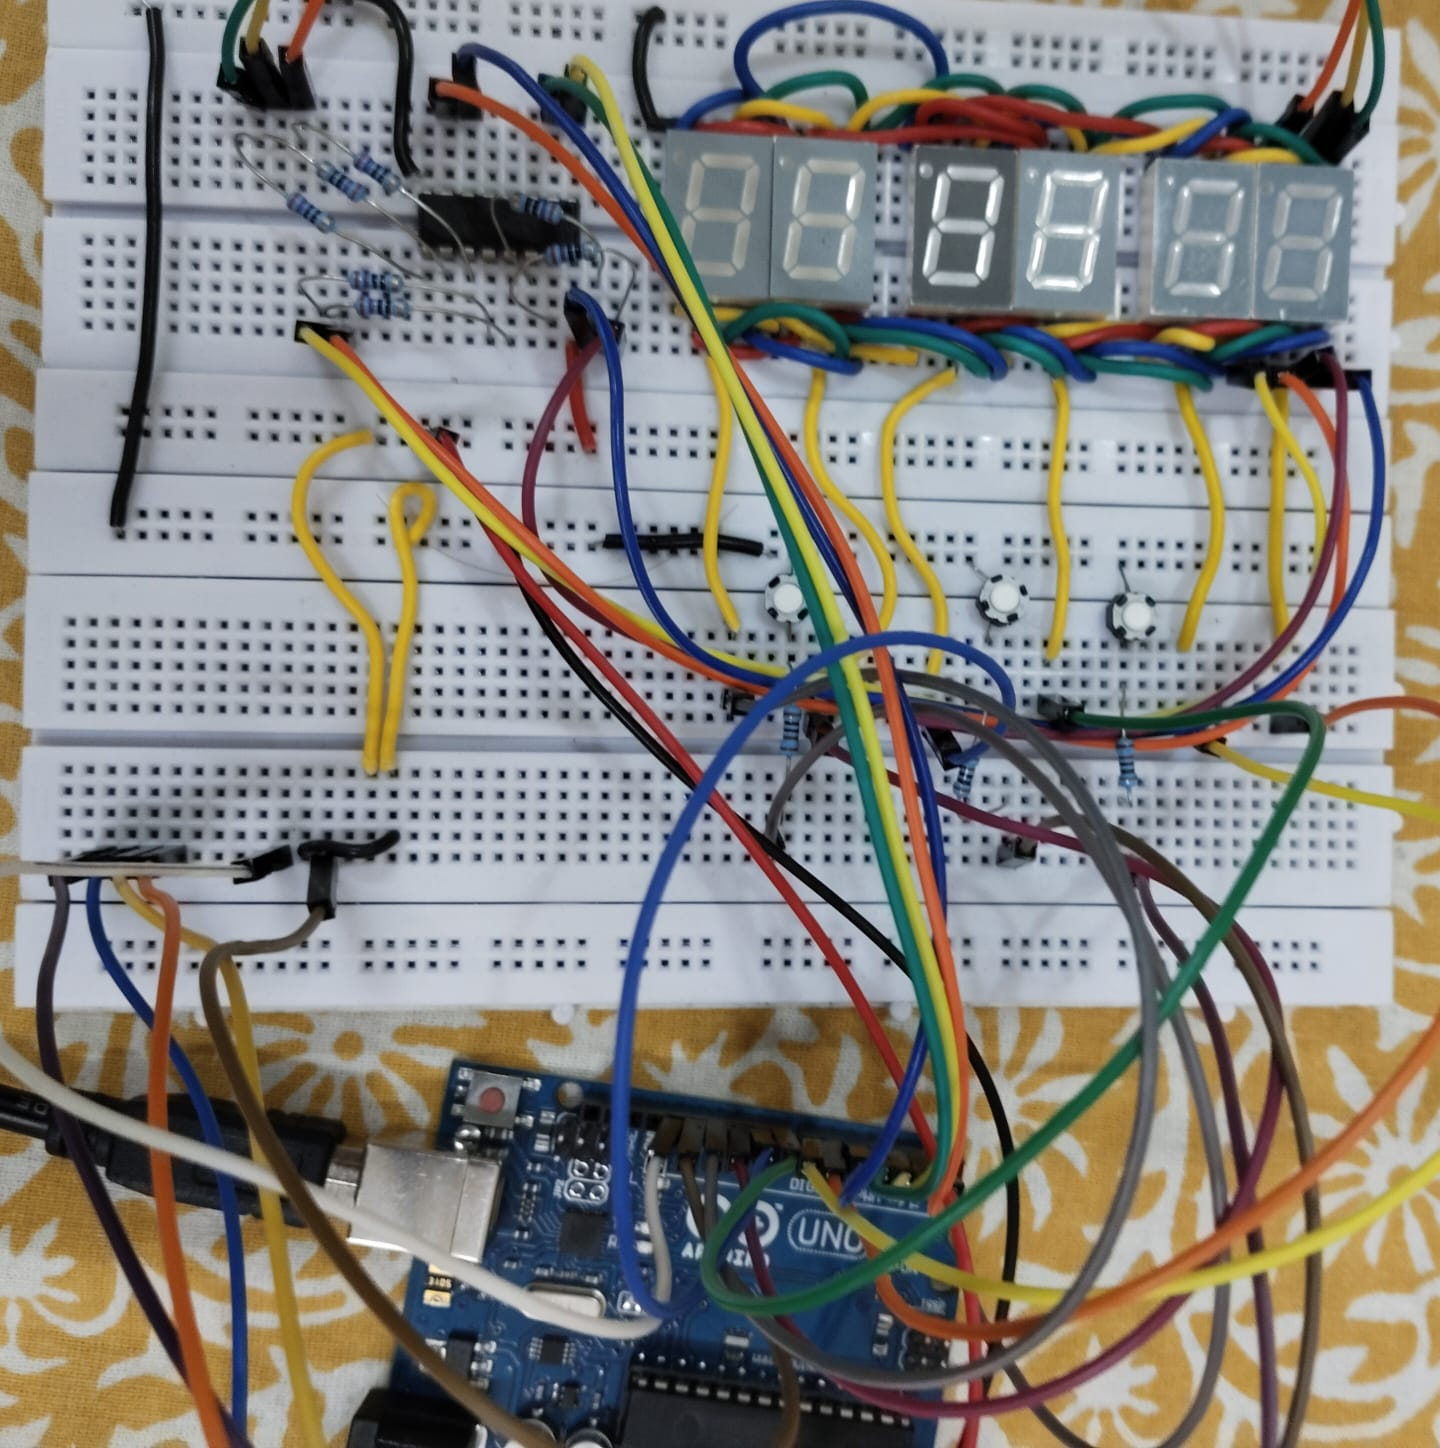
\includegraphics[width=0.4\textwidth]{clk.jpeg}
    \caption*{Digital Clock Circuit}
\end{figure}
\section*{Conclusion}
This project effectively demonstrates how to implement a clock, stopwatch, and timer on an ATmega328P. The use of timer interrupts ensures accurate timekeeping, and the seven-segment multiplexing minimizes GPIO pin usage.

\section*{Reference}
This assignment has been done with the help of dhawal's(ee24btech11015) code.
\end{document}
